\chapter{Exceptions}
	\label{ch:exceptions}

	This chapter explains:
	\begin{itemize}
    \item what an exception is;
    \item why exceptions are useful;
    \item the VB exception facilities.
	\end{itemize}


	\section{Introduction}
		The term 'exception' is used in VB to convey the idea that something has gone wrong: in common terms, an error has occurred. It is an 'exceptional circumstance'. Note that we mean exceptional in the sense of unusual, rather than wonderful! As you will be aware from your use of computers, there are a variety of circumstances in which software can go wrong, but good-quality software should cope with predictable errors in a satisfactory way. For example, here are some awkward situations involving a typical word-processor, with possible (sometimes unsatisfactory) outcomes:
		\begin{itemize}
      \item The system invites you to type a font size as a number, but you type a name. The system could quit and return you to the operating system, or it could ignore your input and leave the font size as it was, or it could display a helpful message and invite you to try again.
      \item You attempt to open a file which cannot be found on disk. The responses could be similar to the previous case.
      \item You attempt to print a file, but your printer is out of paper. Again, this can be predicted, and software can be written to take sensible actions. However, this depends on the printer making its current state available to the software. In actual printers, the software can examine various status bits which indicate out-of-paper, on/offline, paper misfeed, etc.
		\end{itemize}

		\begin{stqb}
			\begin{STQ}
			\item	In the above cases, decide on the best course of action that the word-processor should take.
			\end{STQ}
		\end{stqb}
		Let us look at why we need some form of error notification, and how it might be provided.
		
		When we build software and hardware systems, much of it comes as pre-packaged items, e.g. circuit boards, VB classes and methods. To simplify the design process it is essential to regard these items as encapsulated; we don't want to be bothered with how they work internally, but it is vital that the components which we use provide some indication of error situations. The software can then be written to detect such notification and to take alternative action. But what action to take? This is the difficult bit!
		
		Complex systems consist of a hierarchy of methods (i.e. methods call other methods and so on.) Some exceptions can be handled locally in the method in which they occur, but some more serious cases may need to be passed upstairs to higher-level methods. It depends on the nature of the error. In short, there are different categories of error, which may need to be handled in different places.

		Here is an analogy which illustrates this. Imagine an organization. The managing director starts things happening by giving his managers instructions. In turn, they might instruct programmers and technicians. But things can go wrong. Here are two cases:
		\begin{itemize}
      \item A printer runs out of paper. Normally, the technician handles it. In the rare case that the organization is out of paper, a manager might need to be informed.
      \item A technician trips over a cable and breaks a leg. Exceptions in this category (which might result in legal action etc.) should be handled by the managing director.
		\end{itemize}
		The analogy is that each person doing a job is a method. The job was initiated by someone superior to them. When errors occur, there really needs to be a plan in place saying who handles a particular type of error. The exception facilities of VB allow us to set this up.
		
		Returning now to software. As we said, things go wrong. But do we need a special facility for errors? Surely our If statement will do? We could imagine code of this form:
		\begin{lstlisting}
If something wrong Then
	handle the problem
Else
	handle the normal situation
End If
		\end{lstlisting}
		Here we have used a mixture of English and VB to convey the main point. However, if we have a series of method calls, any of which could go wrong, the logic becomes complex, and can swamp out the normal case. The initially simple sequence of:
		\begin{lstlisting}
MethodA()
MethodB()
MethodC()
		\end{lstlisting}
		would become
		\begin{lstlisting}
MethodA()
If MethodA went wrong Then
	handle the MethodA problem
Else
	MethodB()
	If MethodB went wrong Then
		handle the MethodB problem
	Else
		MethodC()
		If MethodC went wrong Then
			handle the MethodC problem
		End If
	End If
End If
		\end{lstlisting}
		The error cases (which we hope won't happen very often) dominate the logic, and this complexity can make programmers shy away from taking them on. In fact, we will see that the VB exception facilities allow us to stick to the coding for the normal case, and to handle exceptions in a separate area of the program.

		\begin{stqb}
			\begin{STQ}
			\item How could a method return a value which stated whether it worked or not? What if the method returned a value as part of its normal task (i.e. it was a function)?
			\end{STQ}
		\end{stqb}


	\section{The jargon of exceptions}
		Exceptions are created by being thrown, and are detected elsewhere by being caught. VB has \keyword{Throw}, \keyword{Try} and \keyword{Catch} keywords to carry out these tasks. Initially, we will look at the simplest case of catching an exception thrown by a library class.


	\section{A \keyword{Try-Catch} example}
		Here we present a simple program which lets the user enter a \keyword{Double} number representing the side of a square into a text box. The area of the square is then displayed, or an error message, as in:
		\begin{lstlisting}
Area is: 6.25
		\end{lstlisting}
or
		\begin{lstlisting}
Error in side: re-enter
		\end{lstlisting}
		We shall look at the new features introduced in this particular program, then move on to general cases. \Vref{fig:exceptions_square_screen} shows a run with correct input and a run involving an exception. Here is the code:
		\begin{lstlisting}
Private Sub Button1_Click(sender As System.Object,
			e As System.EventArgs)
			Handles Button1.Click
	Dim side As Double
	Try
		side = Double.Parse(TextBox1.Text)
		Label1.Text = "Area is " & CStr(side * side)
				& " sq units"
	Catch exceptionObject As FormatException
		Label1.Text = "Error in side: re-enter"
	End Try
End Sub
		\end{lstlisting}
		\begin{figure}[tbh]
			\centering
			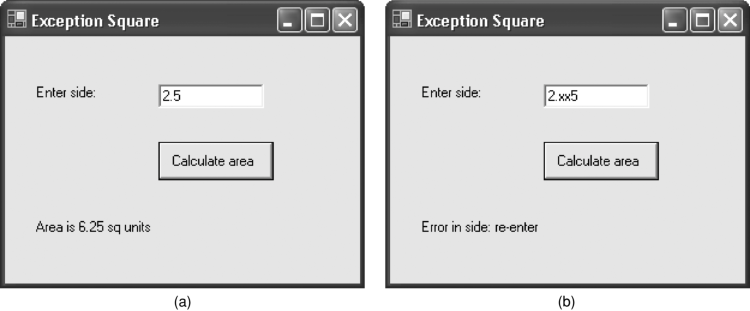
\includegraphics[width=0.9\textwidth]{exceptions_square_screen}
			\caption{The Exception Square program: (a) correct data; (b) incorrect data detected.}
			\label{fig:exceptions_square_screen}
		\end{figure}

		As a relatively minor point, note that in earlier chapters we made use of \keyword{CInt} and \keyword{CDbl} to convert a string of characters into a number, but here we have adopted a more object-oriented approach. In fact, \keyword{CDbl} is not a method of a class: behind the scenes, it makes use of a shared method in the \keyword{Double} class, called \keyword{Parse}. If we consult the documentation on the method, we find that an exception of the class \keyword{FormatException} is thrown by \keyword{Parse} if we supply a string argument containing characters that cannot be converted. (Incidentally, \keyword{Integer.Parse} is used to convert strings to integers). However, the main feature of the example is the introduction of a new statement, which is basically a control structure. It takes the form:
		\begin{lstlisting}
Try
	'a series of statements . . . (the try block)
Catch exceptionObject As FormatException
	'handle the exception in some way . . . (a catch block)
End Try
		\end{lstlisting}
		The concept is that we instruct VB to try to execute a block of statements (the \keyword{Try} block). If it executes without producing an exception, the statements after the word \keyword{Catch} (the \keyword{Catch} block) are ignored, and execution continues after the \keyword{End Try}.
		
		However, if an exception is produced due to some error in the \keyword{Try} block, the \keyword{Try} block stops executing, and we can specify that the \keyword{Catch} block executes by stating the class of exception that we wish to catch. In our example, we consulted the library documentation for \keyword{Double.Parse}, and found that an exception of class \keyword{FormatException} will be produced, i.e. thrown. If another kind of exception occurs, our catch will not be executed, and VB will attempt to find a catch elsewhere in our program which specifies this exception type. We will describe this process in more detail below.
		
		Let us look at the catch block in more detail. In our example, we have:
		\begin{lstlisting}
Catch exceptionObject As FormatException
	Label1.Text = "Error in side: re-enter"
		\end{lstlisting}
		The line containing \keyword{Catch} is rather like the declaration of a method with one argument. We chose to name the argument \keyword{exceptionObject}. When the \keyword{FormatException} is thrown, VB sees that this particular catch can accept an argument of type \keyword{FormatException}. VB deposits an object of type \keyword{FormatException} in \keyword{exceptionObject}. We don't make use of this object in our example, but it can be used to find out more about the exception.
		
		After the \keyword{Catch} block executes, execution continues beneath the \keyword{Catch} block. In many cases, because methods deal with one particular task which cannot sensibly continue after an exception related to that task, it is common to return from the method, as in:
		\begin{lstlisting}
Private Sub Method1()
	Try
		'some code
	Catch exceptionObject As SomeExceptionClass
		'handle it
	End Try
End Sub
		\end{lstlisting}
		In our example program, this is just what is required: the exception handler displays an error message and ends. The user can then enter a new number into the text box.


	\section{Using the exception object}
	When we catch an exception, we already know that something has gone wrong, but additional information comes with the exception object. We can use the \keyword{Message} property and the \keyword{ToString} method, as in:
		\begin{lstlisting}
Catch exceptionObject As FormatException
	MessageBox.Show(exceptionObject.Message)
	MessageBox.Show(exceptionObject.ToString())
		\end{lstlisting}
		\begin{itemize}
      \item The Message property provides a short string containing a descriptive error message. In this example, the message string is:
				The input string is not in a correct format.
			\item The \keyword{ToString} method returns a string containing several lines. The first line is the message as above, and the other lines in the string are a stack trace. It starts in the method where the exception occurs, then works backwards through the methods that were called leading up to the exception. It terminates when a matching \keyword{Catch} is found. Many of these lines will be related to methods within the VB system and libraries, but among them you will find information relating to your code. The key item is the line number within your program. It is here that the exception directly originated, or indirectly originated by calling a method which produced an exception. It is here where you should begin to study your code to find the reason for the exception. \Vref{lst:exceptions_example} shows the output from \keyword{ToString}, with line 139 as the source of the error.
		\end{itemize}
		\begin{lstlisting}[label=lst:exceptions_example,caption=Sample result from \keyword{ToString} with an \keyword{Exception} object.]
System.FormatException: The input string was not in a correct format. 
	at System.Number.ParseDouble(String s, NumberStyles style,NumberFormatInfo info)
	at System.Double. Parse(String s, NumberStyles style,NumberFormatInfo info)
	at System.Double.Parse(String s)
	at ExceptionInserts.Forml.Button5_Click(Object sender,EventArgs e) in C:\mike\homePearVB\vbProjects\Exception Square\ Exception Square.vb:line 139
		\end{lstlisting}


	\section{Classifying exceptions}
		Here we will explore the varieties of exception classes that are provided in the VB library. Basically, the library provides us with a list of exception class names, but if there is no suitably named exception we can also create our own. We will not cover the process of inventing new exceptions, trusting that you will be able to find a suitably named existing one.

		\begin{lstlisting}[label=lst:exceptions_classes,caption=A selection of exception classes.]
Exception
	SystemException
  	ArithmeticException
    	DivideByZeroException
      OverFlowException
    CoreException
    	IndexOutOfRangeException
    FormatException
    	NullReferenceException
    IOException
      EndOfStreamException
      FileNotFoundException
		\end{lstlisting}

		
		Inheritance is used to classify errors into different types. There are a large number of pre-defined exception classes, and \Vref{lst:exceptions_classes} shows a small selection of particularly useful ones.
		
		Here is how to interpret the figure. All exceptions inherit from the \keyword{Exception} class - one such class is the \keyword{IOException} class, which itself is further subclassed, in the sense that \keyword{EndOfStreamException} and \keyword{FileNotFoundException} also inherit from \keyword{IOException}. As the indentation of the names increases, the exceptions become more specific. The reason for this classification system is that we can choose to catch a single exception type (such as \keyword{EndOfStreamException}) or a whole set of exceptions (such as \keyword{IOException}).

		\begin{stqb}
			\begin{STQ}
			\item From \Vref{lst:exceptions_classes} what is the relationship between the \keyword{FormatException} class and the \keyword{IOException} class?
			\end{STQ}
		\end{stqb}
		In \Vref{lst:exceptions_classes} we showed some common exceptions (and we will use some of these when we examine files, in \Cref{ch:files}). But there are many more exception classes. Moreover, merely knowing the names of the exceptions is not the whole story: we need to consider the source of an exception. For each method you use, refer to its documentation. This tells you what it does, what arguments it needs, any exceptions that it might throw, and what classes they belong to.


		\begin{stqb}
			\begin{STQ}
			\item What would be the consequences for the programmer if exceptions were not classified - i.e. the exception structure was just a list of names?
			\end{STQ}
		\end{stqb}


	\section{Multiple \keyword{Catch} blocks}
		Our squaring example only used one \keyword{Catch} block. However, it is possible to use several \keyword{Catch} blocks with one \keyword{Try}. If you do, the rule is that the more specific catch must come first, followed by the more general cases. In the following, we divide 100 by a number entered in a text box. We decided to catch the divide-by-zero exception, then catch any format exceptions, then any remaining system exceptions. The three \keyword{Catch} blocks must be in the order as shown.
		\begin{lstlisting}
Private Sub Button3_Click(sender As System.Object,
				e As System.EventArgs)
				Handles Button3.Click
	Dim bottom As Integer
	Dim top As Integer = 100
	Try
		bottom = Integer.Parse(TextBox1.Text)
		MessageBox.Show(
			"Dividing into 100 gives " & CStr(top \ bottom))
	Catch exceptionObject As DivideByZeroException
		MessageBox.Show("Error - zero:re-enter data")
	Catch exceptionObject As FormatException
		MessageBox.Show("Error in number: re-enter")
	Catch exceptionObject As SystemException
		MessageBox.Show(exceptionObject.ToString())
	End Try
End Sub
		\end{lstlisting}
		Note that if we reversed the order of the last two catches, then a \keyword{FormatException} could never be singled out, because it would be encompassed by the \keyword{SystemException} class.


	\section{The search for a catcher}
		So far, our examples have shown exceptions being produced and handled in the button-click method. But we might choose to handle the exception elsewhere. Here is a re-coding of our example:
		\begin{lstlisting}
Private Sub Button4_Click(sender As System.Object,
				e As System.EventArgs)
				Handles Button4.Click
	MessageBox.Show(
		"This program squares the number in the Text Box . . .")
	Try
		DoCalc()
	Catch exceptionObject As FormatException
		MessageBox.Show("Error: please re-enter")
	End Try
End Sub
Private Sub DoCalc()
	Dim number As Double
	number = Double.Parse(TextBox1.Text)
	MessageBox.Show("val is" & CStr(number * number))
End Sub
		\end{lstlisting}
		The mechanism that is operating is as follows. When an exception happens, VB searches in the current method (\keyword{DoCalc} here) for a \keyword{Catch} block that matches exactly, or that matches a superclass of the exception. If the currently executing method does not provide one, VB abandons its execution, and looks in the method which called the method producing the exception (here, this is the button-click event method). In our example, it finds an appropriate catch here, and executes it. If a matching catch was not found, then the process repeats, looking in the caller of the button-click method. Here we are in the realms of VB system code, but the process is the same. Eventually, the top-most level of code is reached, and the program terminates, displaying a message box. Often this is undesirable - the point of exceptions is to keep the program running when possible.
		
		Note that we do not need to group all our \keyword{Catch} blocks together in one method. The following code shows one exception being caught in \keyword{DoCalc}, and any others being caught in the button-click method.
		\begin{lstlisting}
Private Sub Button1_Click(
					sender As System.Object,
					e As System.EventArgs)
					Handles Button1.Click
	MessageBox.Show(
		"This program squares the number in the Text Box . . .")
	Try
			DoCalc()
	Catch exceptionObject As Exception
			MessageBox.Show("Exception thrown from DoCalc()")
	End Try
End Sub
Private Sub DoCalc()
	Dim number As Double
	Try
			number = Double.Parse(TextBox1.Text)
			MessageBox.Show("Square is" & CStr(number * number))
	Catch exceptionObject As FormatException
			MessageBox.Show("Incorrect number: re-enter")
	End Try
End Sub
		\end{lstlisting}
		Here is a more general description of the mechanism. Assume that in a particular run of a program, \keyword{Method1} calls \keyword{Method2}, which in its turn calls \keyword{Method3}. (We do need to state that this is a particular run of a program, because the pattern of execution of methods might depend on data that the user enters.) Anyway, this run produces an exception in \keyword{Method3}. The process is:
		\begin{itemize}
      \item The execution of \keyword{Method3} is abandoned.
      \item If there is a matching \keyword{Catch} block in \keyword{Method3}, it is used and, eventually, execution of the method resumes after the \keyword{End Try}. Bear in mind that a \keyword{Catch} block matches if it specifies the particular exception, or a superclass of the exception.
				If, on the other hand, \keyword{Method3} does not have a matching \keyword{Catch} block, VB looks 'upward', in the method which called \keyword{Method3} (\keyword{Method2} here). If a matching \keyword{Catch} block is found, it is executed, and execution continues beneath the \keyword{End Try}.
      \item If \keyword{Method2} does not contain a matching catch, then its calling method (\keyword{Method1}) is examined. This process of looking backwards through the calls is termed 'propagating' the exception. If no catcher is found, the program eventually terminates, displaying details of the exception.
		\end{itemize}


	\section{Throwing - an introduction}
	Here we will code a method which throws an exception. The task of the method is to convert a string containing either \keyword{"ten"}, \keyword{"hundred"} or \keyword{"thousand"} to its equivalent integer. To make this method useful in a range of situations, we will throw an exception. This allows the caller of the method to decide on the action to take. We will opt to throw an instance of the \keyword{FormatException} class. Here is the code:
		\begin{lstlisting}
Private Sub Button6_Click(sender As System.Object,
			e As System.EventArgs)
			Handles Button6.Click
	MessageBox.Show(CStr(WordToNumber("hXndred")))
End Sub
Private Function WordToNumber(word As String)
				As Integer
	Dim result As Integer = 0
	If word = "ten" Then
		result = 10
	ElseIf word = "hundred" Then
		result = 100
	ElseIf word = "thousand" Then
		result = 1000
	Else	
		Throw New FormatException("Wrong input: WordToNumber")
	End If
	Return result
End Function
		\end{lstlisting}
		
		The \keyword{Throw} statement is often executed as the result of an If: it creates a new instance of the specified exception class, and initiates a search for a matching catch. When creating a new exception, it is possible to provide an alternative message string, which the catcher can obtain by using the \keyword{Message} property.


	\section{Handling - some possibilities}
		Approaches to handling depend on the nature of the exceptions and on the nature of the program they occur in. We will look at two exceptions:
		\begin{itemize}
      \item the \keyword{FormatException};
      \item the \keyword{IndexOutOfRangeException}.
		\end{itemize}
		We made use of \keyword{FormatException} in our squaring program and adopted the handling approach of displaying an error message, asking the user to try again. This is possible (and sensible) here because the data comes directly from the user, who is interacting with the program. However, if the reason for the error was incorrect data in a database (perhaps a list of exam marks) we might not wish to offer the user a chance to try again. Instead, we might display a message suggesting that the user contacts the creator of the database, and then terminate the program.
		
		Let us look at possibilities for \keyword{IndexOutOfRangeException}. It might come from code such as:
		\begin{lstlisting}
Dim a(9) As Integer
Dim n As Integer
For n = 0 To 10
	a(n) = 25
Next
		\end{lstlisting}
		This is different. Catching it is fine, but then what? The problem was not caused by user input. The \keyword{For} produces a loop from 0 to 10 inclusive, and thus attempts to access \keyword{a(10)}: we should have made the loop run from 0 to 9. This is a programming mistake, which should really have been found at the testing stage. It needs fixing by debugging and re-compiling.
		
		So, is it worth catching \keyword{IndexOutOfRangeException} and also \keyword{ArithmeticException} cases, which could originate from the misuse of commonplace facilities such as arrays and division? One approach is to ignore them. The search for a catcher will fail, and a message will appear on the screen. The program needs debugging and further testing should be performed.


	\section{\keyword{Finally}}
		The full \keyword{Try} statement has an additional facility, namely \keyword{Finally}. Here is an example in a mixture of English and VB. Assume that the task falls into two parts: the main task, followed by some termination code that must be performed whether or not an exception happens in the main calculation. Without \keyword{Finally}, we would code this as:
		\begin{lstlisting}
Try
	main task
	termination code
Catch exceptionObject As FormatException
	display an error message
	termination code
End Try
		\end{lstlisting}
		The use of \keyword{Finally} helps us to avoid duplicating the termination code, which we require to be performed in every situation, as in:
		\begin{lstlisting}
Try
	main task
Catch exceptionObject As FormatException
	display an error message
Finally
	termination code
End Try
		\end{lstlisting}
		Code that is placed in the \keyword{Finally} section will always be performed, whether or not an exception occurs. The \keyword{Finally} code will even be performed if our \keyword{Catch} does not match the exception, or if the \keyword{Try} block executes a \keyword{Return} or throws an exception itself.


	\section{Programming principles}
		\begin{itemize}
      \item When writing general-purpose methods (where their future use might be unknown) you should throw exceptions, rather than terminating the program or concealing a possible error.
      \item An exception changes the order in which statements are obeyed, hence it is a form of control structure. But exceptions should not be used for normal cases. 
				For example, if the user is entering a series of names, and will type \keyword{"END"} at the end of the list, then this is not an error. It should be handled by a \keyword{While} or \keyword{If}, rather than treating it as an exception.
		\end{itemize}


	\section{Programming pitfalls}
		\begin{itemize}
      \item Allowing an exception to be thrown from a method, when it can sensibly be handled locally.
      \item Attempting to catch and process exceptions such as \keyword{ArithmeticException} and \keyword{IndexOutOfRangeException}. In most cases, there is little that can be done. Catching such errors can conceal them, when instead the programmer needs to know about them.
		\end{itemize}


	\section{Grammar spot}
		\begin{itemize}
      \item The basic try-catch structure is:
				\begin{lstlisting}
Try
	'a series of statements
Catch exceptionObject As SomeExceptionClass
	'handle the exception
End Try
				\end{lstlisting}
      \item A \keyword{Finally} section can precede the \keyword{End Try}.
      \item An exception can be thrown by:
				\begin{lstlisting}
Throw New SomeExceptionClass("error message")
				\end{lstlisting}
		\end{itemize}


	\section{New language elements}
		\begin{itemize}
      \item \keyword{Try} and \keyword{End Try}
      \item \keyword{Catch}
      \item \keyword{Finally}
      \item \keyword{Throw}
      \item the exception hierarchy.
		\end{itemize}


	\section{New IDE facilities}
		There are no new IDE facilities in this chapter.


	\section{Summary}
	\begin{itemize}
      \item An exception is an unusual situation.
			\item Exceptions are instances of classes, created by \keyword{New}.
      \item \keyword{Try} blocks are used to surround code which could throw an exception.
      \item A \keyword{Catch} block can pick up one exception type or a class containing several exceptions.
			\item The inheritance tree of the class \keyword{Exception} (\Vref{lst:exceptions_classes}) shows you the main exceptions you will have to deal with and which class they are in.
      \item Exceptions within the \keyword{SystemException} class are difficult to fix up, and in many cases can be intentionally ignored.
	\end{itemize}


	\section{Exercises}
		\begin{EXE}
		\item	Write a program which provides two textboxes for the input of integer values \keyword{a} and \keyword{b}. Display the result of \keyword{a\textbackslash b} and \keyword{b\textbackslash a}. (Recall that \textbackslash performs integer division.) Incorporate exception handling for zero and non-numeric input text box values.
			\item	Write a method which solves quadratic equations. Normally, there are two real roots. The method call should take the form:
				\begin{lstlisting}
Solve(a, b, c, root1, root2)
				\end{lstlisting}
				where the roots are passed back through reference parameters. The formulae to calculate the roots are:
				\begin{lstlisting}
root1 = (-b+Math.Sqrt(b*b-4*a*c))/(2*a)
root2 = (b-Math.Sqrt(b*b-4*a*c))/(2*a)
				\end{lstlisting}
				In the case when the discriminant b*b-4*a*c is negative, throw an \keyword{ArithmeticException} with a suitable message. Write a calling method which catches your exception.
			\item If you know the length of the three sides of a triangle, the area can be calculated by:
				\begin{lstlisting}
area = Math.Sqrt(s * (s - a) * (s - b) * (s - c))
				\end{lstlisting}
	where
				\begin{lstlisting}
s = (a+b+c)/2
				\end{lstlisting}
				Write a method for calculating and returning the area. Make it throw a suitable exception (with a message) message when the three lengths cannot form a triangle. Write a calling method which catches your exception.
			\item	Write a program which inputs three strings from three text boxes, representing day number, month number and year. For example, the strings "23", "5", "2007" represent the 23rd of May 2007. Produce a suitable error message if an item is non-numeric, missing completely or specifies an impossible date. Ignore leap years.
			\item Write a program which calculates compound interest. The user inputs the initial amount ($i$), the (fixed) interest rate per year ($r$) as a percentage value (a \keyword{Double}), and the number of years to run ($n$). Display the final amount ($f$). Provide full error-checking on input data. Here is the formula:
				\begin{equation*}
					f = i \left[ 1 + \frac{r}{100}\right]^n
				\end{equation*}
			\end{EXE}

		\begin{stab}
			\begin{enumChapter}
				\item In the first two cases, quitting the program would be a poor course of action. A more useful response is to display some sort of error indication, and allow the user either to have another go or to abandon the selection of the item. In the third case, the complication is that the printer may run out of paper part-way through a print. The user needs to be informed of this, and may be provided with options to abandon the print request or, assuming that paper has been loaded, continue printing from a particular page.
				\item	If the method was not a function, it would be possible to use Return to pass back a \keyword{Boolean} value. The method would now be called like a function, as in:
					\begin{lstlisting}
Dim error As Boolean
error = DoTask()
					\end{lstlisting}
					However, if a value is already being returned, a reference parameter would have to be used, as in:
					\begin{lstlisting}
Dim error As Boolean
biggestValue = Bigger(44, 55, error)
If error = True Then
	... etc.
					\end{lstlisting}
					Either approach is inconvenient.
				\item	\keyword{FormatException} inherits from \keyword{SystemException} (which in its turn inherits from Exception). \keyword{IOException} inherits from \keyword{Exception}. There is no relationship between the two classes apart from the fact that they inherit from \keyword{Exception}, as do all the exception classes.
				\item	Catching an exception which had never been inherited from would be as before. But consider the case of catching every exception. We would need a huge list of catches.
			\end{enumChapter}
		\end{stab}
